\documentclass[10pt,twocolumn]{article}
\usepackage[margin=0.9in,columnsep=0.33in]{geometry}
\usepackage{amsmath,amssymb}
\usepackage{graphicx}
\usepackage{booktabs}
\usepackage{fontspec}
\usepackage{xeCJK}
\setCJKmainfont{Songti SC}
\usepackage[hidelinks]{hyperref}
\setlength{\parindent}{0pt}
\setlength{\parskip}{4pt plus 1pt}
\title{\textbf{Mechanical Judges as an Exact Reference: Measuring LLM Judge Reliability on the Formalizable Core}}
\author{Anonymous (double-blind)}
\date{}
\begin{document}
\maketitle
\begin{abstract}
LLM judges are default in automated evaluation, yet their reliability on the formalizable core — where the correct answer is a numeric value or spec-constrained quantity — has not been measured against an exact reference. We measure it. On 67 real model outputs across 10 tasks, a 27b LLM judge under three prompt variants emits unparseable output on 52–84\% of checkpoints (Wilson 95\% CI excluding 0), and on the checkpoints it does parse its verdicts are stratified by reference quality: on the exact-reference core it agrees with the mechanical reference 94.5\% of the time (4/73 flip), while on the heuristic-reference stratum it diverges 80.5\% (128/159) — the LLM judge is redundant on the exact core (confirming what the exact reference already gives) and the more capable judge on the heuristic residual. A mechanical judge (symbolic comparison or spec-driven regex) fails on 0/67 by construction. We isolate the mechanism: complexity lengthens the judge's reasoning chain, exhausting max\_tokens and truncating the verdict — not attention dilution; prompt phrasing spans 31.4pp across variants, V3 best at 52.2\%. We certify the task set against guessing via a model-agnostic bound (P(all-correct by guess) ≤ 3.3×10⁻⁵) and show prompt optimization trades one checkpoint dimension for another. The contribution is the *reference*: on the formalizable core a mechanical judge is exact on calc checkpoints, free, and reproducible, and is the appropriate default there, with LLM judgment reserved for the non-formalizable residual.
\end{abstract}

\section{Introduction}
LLM-as-a-judge has become the default evaluation mechanism for LLM systems: it scales where human evaluation cannot, and it is now embedded in benchmarking pipelines, preference-label generation, and safety review. A rapidly growing literature (an arXiv search for "LLM judge" returns over 1,000 papers submitted in 2026 alone) has established that these judges are unreliable — they exhibit position bias, verbosity bias, self-preference, and instruction sensitivity. What this literature has not addressed is a more basic question: *on the subset of evaluation targets that are mechanically checkable, is an LLM judge even necessary?*


This question matters because the reliability of the judge silently bounds the validity of the entire evaluation pipeline. An automated agent-evaluation harness scores thousands of outputs per day; if the judge fails to emit a parseable verdict on half of them, the pipeline is not producing a noisy score — it is producing *no score* on half the data, and every aggregate reliability metric computed over the parseable subset is conditioned on a selection that the metric itself does not report. The failure is worse than a biased scorer: it is a scorer that is intermittently absent, and the absence is correlated with the difficulty of the item being scored (the harder the checkpoint, the more likely the judge's reasoning chain overruns its token budget and truncates).


We study this question on the formalizable core — the part of an evaluation target whose correctness reduces to a finite set of numeric or boolean checkpoints with a known ground truth (a gold value and a tolerance, or a spec-driven keyword/forbidden pattern). For GPU systems questions, this core includes derived quantities (throughput, KV-cache budget, ridge-point classification) and datasheet-anchored facts; for math/physics questions it includes closed-form values. The core is exactly the part where a mechanical judge — SymPy symbolic comparison for numeric checkpoints, spec-driven regex for boolean ones — is exact, free, and reproducible by construction. Our working hypothesis is that on this core the LLM judge is not merely unnecessary but actively harmful: it adds a failure mode (format truncation) that the mechanical judge does not have, and it adds noise (verdict flips) that the mechanical judge does not have.


Our contribution. Against a mechanical judge as the exact reference, we measure a 27b LLM judge on 67 real model outputs across 10 tasks (7 full-rank, 3 rank-deficient) under three prompt variants (201 judge calls total). We find:


1. Format reliability fails (F1). The LLM judge emits unparseable output on 52–84\% of calls depending on prompt variant; the mechanical judge fails on 0\% by construction. The failure is content-driven (task type / gold complexity), not a length threshold: full-rank tasks fail 7/7 across the entire length range.


2. The mechanism is attributable and unstable (F2). Controlled re-judging, output-tail inspection, and a 5-rep determinism probe show the mechanism is a single causal chain — input complexity → longer reasoning chain → collision with max\_tokens → JSON truncation — not attention degradation. Three behavior classes: truncation-recoverable (Q01/Q02/Q06), convergence failure (Q03/Q05, the model cycles and cannot emit a verdict even with more tokens), and a borderline class (Q04) that flips run-to-run at temperature 0 — the same input at the same temperature alternates between a 74-char JSON and a 2600-char reasoning chain. The root cause is instruction-following non-determinism; the LLM judge's format reliability is not merely low, it is unstable.


3. Verdict accuracy is stratified by reference quality (F3). On the parseable subset the LLM judge agrees with the exact mechanical reference 94.5\% of the time on the exact-reference core (4/73 flip) but diverges 80.5\% on the heuristic-reference stratum (128/159) — redundant on the core, more capable on the residual.


4. The task set resists guessing (F4). F1–F3 ask whether the judge can be trusted; F4 asks whether the *test* can be trusted. Under an explicit random-guess model, the probability of guessing all checkpoints correct is bounded analytically (1.2e-10 to 3.3e-5); 2000 seeded simulations produced 0 full-guess successes (consistent with, but underpowered to verify, the bound). The bound is model-agnostic.


5. Prompt optimization is not free (F5). A three-arm behavioral experiment shows that fixing one checkpoint dimension (c1: 33\%→100\%) induces a side effect on another (c3: 100\%→77\%, via induced conditional-enumeration / hedging behavior).


Positioning. The closest prior work is the Judge Reliability Harness (Dev et al. 2026), which measures a judge's robustness to *input* perturbations (formatting, paraphrasing, verbosity, label flip). We measure a judge's *output* format reliability — the rate at which it fails to emit a parseable verdict at all — a failure mode JRH does not instrument. Where the reliability literature reports correlations ("reliability varies with X"), we attribute failures to actionable mechanisms (truncation vs complexity vs instruction-following) with direct engine evidence. Where prior work relies on human annotation or perturbation tests as ground truth, our mechanical reference is exact and free on the formalizable core. Where no prior work provides a guarantee that high scores are not guessable, we give a model-agnostic analytic bound.


Implication. On the formalizable core, the mechanical judge should be the default: it is exact, free, reproducible, and its failure mode (none) is known. LLM judges remain appropriate for the non-formalizable residual — explanation quality, style, argument structure — where no mechanical reference exists.


Paper structure. §2 describes the task set, the two judges, and the measurement protocol. The findings section reports five findings (F1–F5): format reliability (F1), mechanism attribution (F2), verdict accuracy (F3), the anti-guessing bound (F4), and prompt side effects (F5). A related-work section positions the contribution against the LLM-judge-reliability literature. An implications-and-limitations section closes the paper. Task construction and gold-derivation traces are in the appendix.

\section{Setup \& Method}
\#\#\# 2.1 Task set


Ten tasks: 7 full-rank (Q01–Q07) and 3 rank-deficient (Q08–Q10). Domains: GPU systems (7), math (1), physics (1). Each task carries 4–5 checkpoints (47 total).


Full-rank tasks are self-contained: the prompt provides all information needed to derive every checkpoint's gold value. Gold values are derived symbolically (SymPy 1.14.0) from the prompt's given quantities, or anchored to public datasheets (NVIDIA H100/H200 specs). Checkpoint types: calc (numeric, tolerance 2\% or exact-integer), fact (numeric or textual, datasheet-anchored), bool (spec-driven keyword/forbidden-pattern). A representative example (Q01): a 32B FP8 model served on a single H100 SXM (80 GB HBM3, 3.35 TB/s) at batch 16 and context 12288 — five checkpoints form a dependency chain: c1 the H100 datasheet TDP (700 W), c2 the KV-cache bytes per token (64·8·128·2, tolerance 2\%), c3 the bytes moved per decode step (weights + batch·ctx·kv\_per\_token, depends on c2), c4 the aggregate decode throughput at 85\% of HBM bandwidth (depends on c3), c5 the joules per generated token (depends on c1 + c4). The chain makes the task internally consistent: each downstream checkpoint is only derivable if the upstream one is correct, which gives the mechanical judge a non-trivial dependency structure to check.


Rank-deficient tasks deliberately withhold information: Q08 omits the per-GPU HBM capacity (the model must either commit to a value from memory or flag the gap); Q09's retrieved spec excerpt is missing a row the question requires; Q10 presents two contradictory sources (vendor datasheet 3.35 TB/s vs blog 2.0 TB/s). These probe whether the model *knows what it doesn't know* — the rank-deficient axis. The prompt constrains the allowed source ("the only source you are allowed to use is this retrieved spec excerpt"), so supplementing with external facts is a scored violation, not a recovery. The correct behavior on a rank-deficient task is a two-part answer: (i) name the missing quantity (textual-gold checkpoint), and (ii) still compute the quantities that are derivable from the given information (calc checkpoints). This design makes the rank-deficient tasks a calibration probe: a model that fabricates the missing value fails the textual checkpoint; a model that refuses to compute anything fails the calc checkpoints; only a model that separates "what I know" from "what I don't" passes both.


Task construction and gold verification. Every gold value is derived by a SymPy expression at construction time and self-checked (the expression must evaluate to the stated gold within tolerance before the task is accepted). This makes the mechanical reference exact by construction: there is no human annotation step, no tolerance negotiation, and no "close enough" judgment. The full gold-derivation trace for all 47 checkpoints is in Appendix A.


\#\#\# 2.2 Judges


Mechanical judge. Each checkpoint is evaluated deterministically:


\begin{itemize}
  \item calc (tol > 0): SymPy evaluates the gold expression; the model's extracted value passes iff |v−g|/|g| < tol.
  \item calc (tol = 0, integer): exact match after SymPy evaluation.
  \item fact (numeric): same as calc with the fact's tolerance.
  \item fact (textual): spec-driven keyword match.
  \item bool: spec-driven keywords (any present → pass) and forbidden\_numbers/forbidden\_patterns (any present → fail). Supports "pass-by-absence" checkpoints (e.g., "must not output tok/s").
\end{itemize}


The mechanical judge is exact by construction: its only failure mode is a bug in the spec, which is caught by a SymPy self-check at task-construction time (Appendix A). One scope caveat, reported separately throughout: on the rank-deficient *textual-gold* checkpoints (naming a missing quantity), the mechanical reference is a regex heuristic, not an exact symbolic check. We flag every result that depends on this heuristic (F3 scope note) and show that the LLM judge is reliable on the exact-reference core (it agrees with the exact reference ≈95\% of the time) and diverges on the heuristic stratum, where the mechanical reference is the weaker instrument.


LLM judge. A 27b model (Qwen3-27B, local vLLM deployment, temperature 0) is prompted to judge each checkpoint and emit a JSON verdict \{"c1": true/false, ...\}. The judge is the same model family as the model being evaluated (27b judging 27b), which is the realistic deployment configuration for a cost-constrained evaluation pipeline and makes the result directly applicable to that setting. Three prompt variants:


\begin{itemize}
  \item V1\_strict: "You are a strict numeric grader. Judge each checkpoint right/wrong. tolerance=0.02 checkpoints: within 2\% of gold = right; tolerance=0 (integer): must equal gold exactly, off-by-one = wrong. Output JSON only: \{\"checkpoint\_id\": true/false\}. No explanation."
  \item V2\_loose: relaxed tolerance phrasing + "be lenient on rounding".
  \item V3\_engineer: structured engineering rubric + "show your check before the JSON".
\end{itemize}


The three variants span the prompt-design space a practitioner would realistically use: a strict contract (V1), a lenient phrasing (V2), and a structured rubric that asks the judge to show its work (V3). The variant is the only thing that changes between the three measurement arms; the model, temperature, and task set are held fixed.


Default max\_tokens=500 (the deployment default; the truncation mechanism in F2 is measured at this budget). The choice is deliberate: 500 is a common production default for judge calls (it bounds cost and latency), and the truncation mechanism we measure is precisely the failure mode that this budget induces.


\#\#\# 2.3 Measurement protocol


\begin{itemize}
  \item Format reliability = fraction of judge calls emitting unparseable output (no valid JSON verdict object).
  \item Flip rate = on parseable calls, fraction of checkpoints where LLM verdict ≠ mechanical verdict.
  \item Mechanism attribution: (i) max\_tokens 500→2000 re-judging of failure cases (truncation recovery rate); (ii) engine finish\_reason and completion\_tokens (direct truncation evidence); (iii) partial correlation of input length vs failure controlling for output length (independent complexity effect); (iv) within-checkpoint-count stratification (gold-complexity vs checkpoint-count attribution).
  \item Guessing bound: explicit random-guess model (continuous: U[0.5g, 2g], hit prob 2·tol/1.5; integer: U[g±50], hit prob 1/101; textual: 1/100 conservative), analytic product bound + Monte Carlo (N=2000, seed=42).
  \item Three-arm behavioral experiment (rank-deficient only, n=10/arm): A\_baseline (no reminder), B\_remind (commitment reminder), B'\_remind (commitment + conditional-enumeration inducement). c3 scored under two criteria: strict (commit to a single value; conditional enumeration = miss) and lenient (hedging-word exemption per sentence window).
\end{itemize}


\#\#\# 2.4 Deployment


27b model served via vLLM at a local endpoint; no weight updates. All judge calls at temperature 0. Task construction and gold verification use SymPy 1.14.0; the full gold-derivation trace is in Appendix A. The judge and the evaluated model run on the same deployment, so the measurement is a within-system comparison: the only difference between the two "judges" is the verifier (mechanical vs LLM), not the model or the serving stack.

\section{Findings}
\begin{figure}[t]
\centering
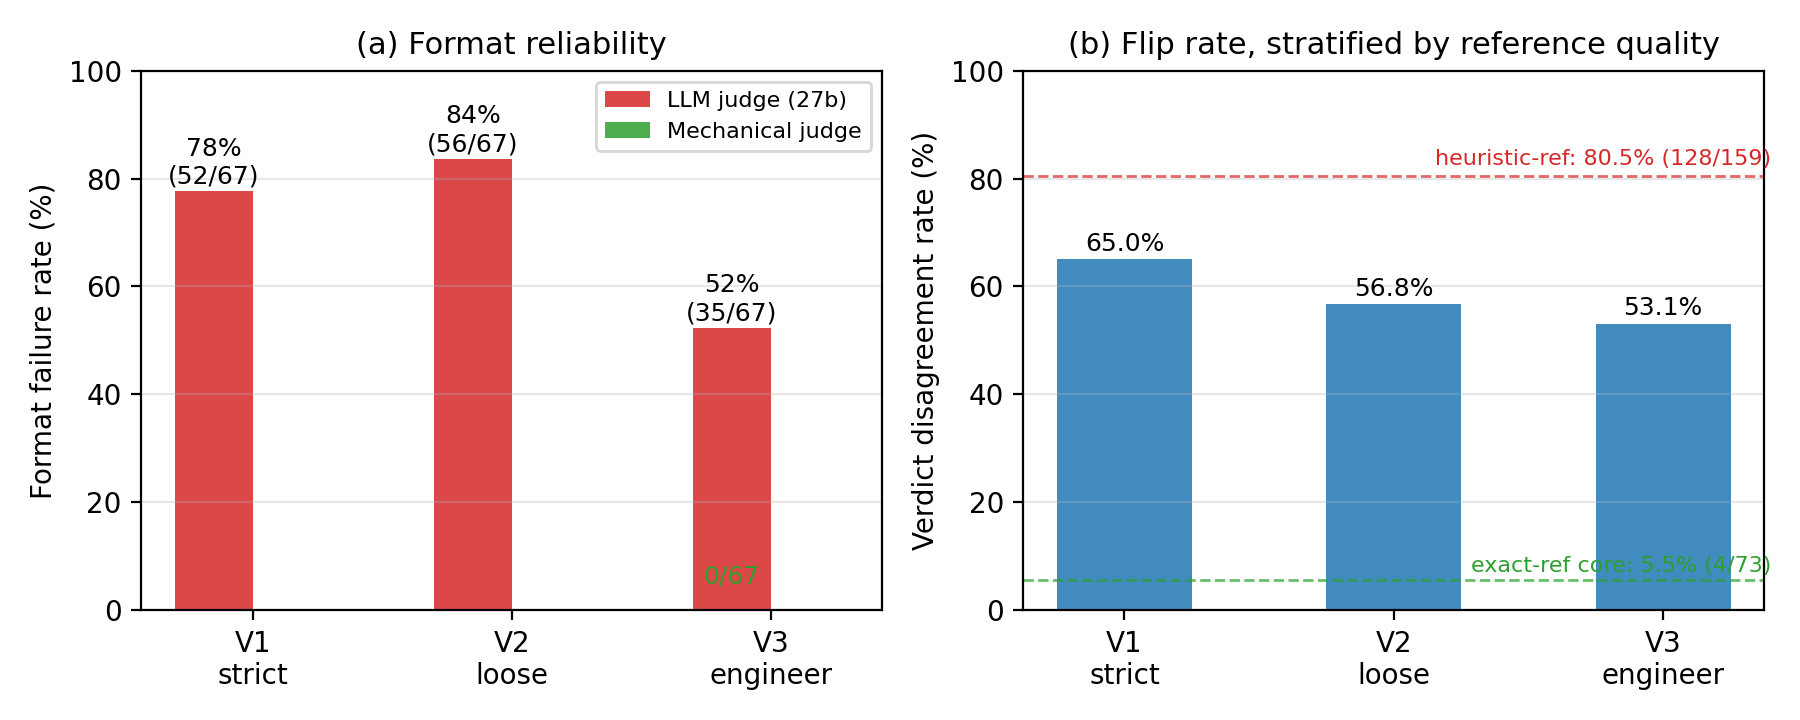
\includegraphics[width=\columnwidth]{figures/fig1-format-reliability.png}
\caption{Panel (a): format failure rate (bars) across the three prompt variants; the mechanical judge fails on 0\% of calls. Panel (b): verdict flip rate (bars, pooled across reference strata) with the two stratum-level reference lines — exact-reference core 5.5\% (4/73) and heuristic-reference 80.5\% (128/159).}
\end{figure}

\begin{figure}[t]
\centering
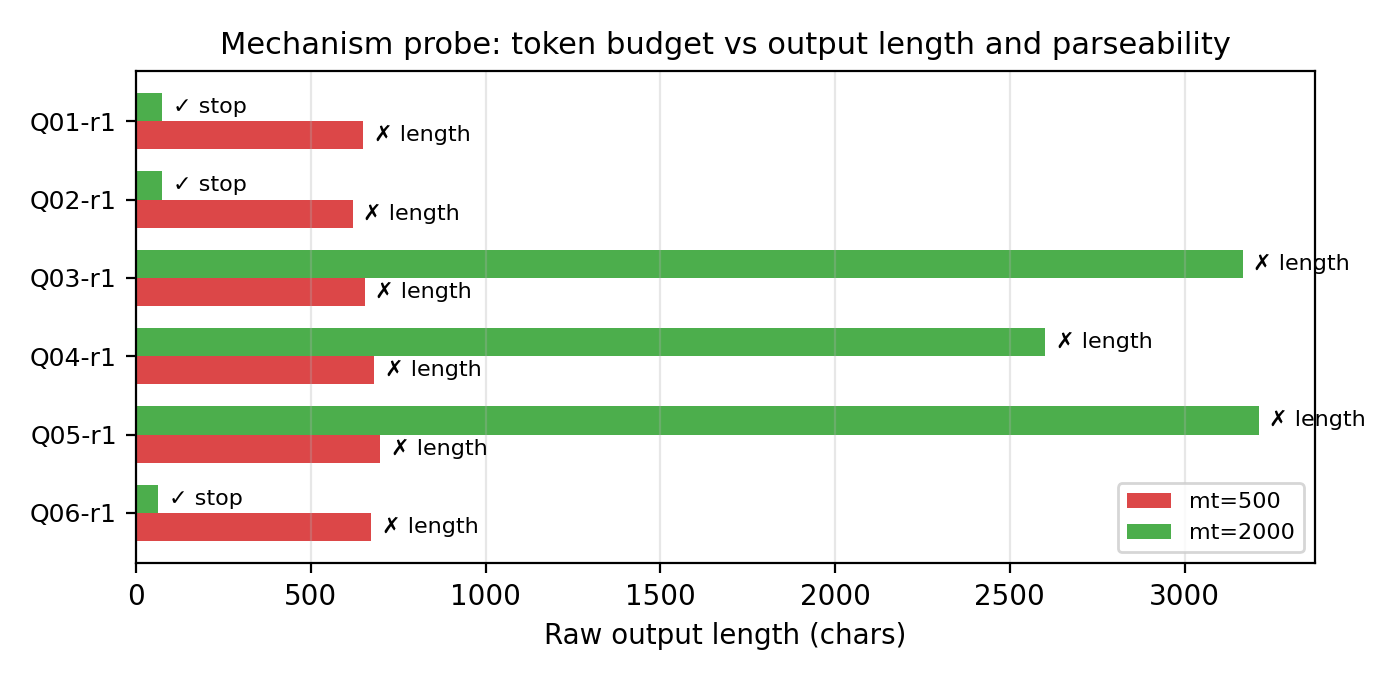
\includegraphics[width=\columnwidth]{figures/fig2-mechanism.png}
\caption{Mechanism probe: the six V1 failure cases re-judged at max\_tokens 500 vs 2000. Recovery is determined by whether the reasoning chain converges, not by max\_tokens itself.}
\end{figure}

\begin{figure}[t]
\centering
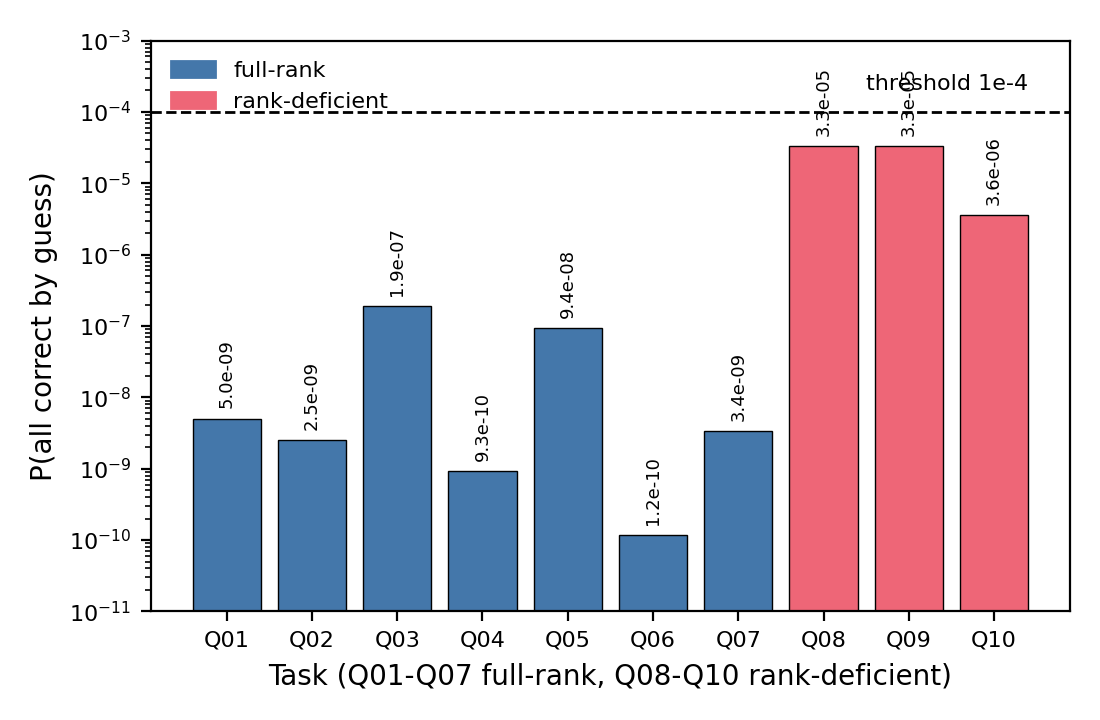
\includegraphics[width=\columnwidth]{figures/fig3-guess-bound.png}
\caption{Analytic upper bound on the probability of guessing all checkpoints correct, per task. Full-rank tasks (blue) sit at 1e-10 to 1e-7; rank-deficient tasks (red) at 1e-6 to 3.3e-5. All are far below the 1e-4 threshold. 2000 seeded simulations produced 0 full-guess successes — consistent with the bound, but underpowered to verify it at the most-guessable task (expected 0.07 successes).}
\end{figure}

\begin{table}[h]
\centering
\begin{tabular}{llll}
Judge & Format failure (Wilson 95\% CI) & Verdict flip vs mechanical (CI) & Parseable n \\
V1 strict & 77.6\% (52/67, [66,86]) & 65.0\% (39/60, [52,76]) & 15 \\
V2 loose & 83.6\% (56/67, [73,91]) & 56.8\% (25/44, [42,70]) & 11 \\
V3 engineer & 52.2\% (35/67, [40,64]) & 53.1\% (68/128, [45,62]) & 32 \\
Mechanical & 0\% (0/67) & 0\% (by construction) & 67
\end{tabular}
\end{table}


Flip denominator = parseable checkpoints where both judges rendered a verdict. Pooled across reference strata; stratified: exact-reference core 4/73 (5.5\%), heuristic-reference 128/159 (80.5\%) — see F3.


We measure format reliability as the rate at which an LLM judge emits unparseable output on inputs where a mechanical judge succeeds by construction. On 67 real 27b outputs across 10 tasks (7 full-rank, 3 rank-deficient), three prompt variants (V1\_strict, V2\_loose, V3\_engineer) yield format failure rates of 77.6\% (52/67, Wilson 95\% CI [0.663, 0.859]), 83.6\% (56/67, CI [0.729, 0.906]), and 52.2\% (35/67, CI [0.405, 0.637]) respectively. The mechanical judge, which evaluates each checkpoint by SymPy symbolic comparison or spec-driven regex, fails on 0/67 (0\%) by construction.


The failure is not a smooth function of output length; it is confounded with task type. Full-rank tasks (Q01–Q07, complex symbolic gold) fail 7/7 across the full length range (385–7210 chars) — including the shortest output in the set (Q07, 385 chars). Rank-deficient tasks (Q08–Q10, where the model often emits a short "flag the gap" response) fail 45/60, with a genuine length effect *within* the group: Q09's nine 435-char outputs all parse, while its 1707–1848-char outputs mostly fail. An apparent "604-char threshold" in the pooled data is an artifact of this task-type confound (the two task types happen to occupy different length bands), not a hard length boundary. The mechanism is content-driven, not length-driven: complex gold values force the judge into a long reasoning chain that exhausts the token budget (F2), while short gap-flagging responses let the judge emit a verdict quickly.


Claim. No prompt phrasing brings a 27b LLM judge to usable format reliability on the formalizable core: even the best variant (V3) fails 52\% of the time, versus 0\% for the mechanical judge.


Pipeline impact. In an automated evaluation harness, a 52–84\% format failure rate is not a noisy score — it is a *missing* score on half to four-fifths of the data. Every aggregate reliability metric computed over the parseable subset is conditioned on a selection that the metric itself does not report, and the selection is correlated with item difficulty (the harder the checkpoint, the more likely the judge's reasoning chain overruns its budget). The pipeline is not producing a biased estimate; it is producing no estimate on the hardest items, which is exactly where the estimate is most needed.


We attribute format failures with a controlled re-judging probe (max\_tokens 500→2000) plus engine finish\_reason and output-tail inspection. The probe (v2, 6 V1 failure cases) shows the mechanism is not attention degradation (which would make verdicts more *wrong*) but token-budget exhaustion by the reasoning chain.


The causal chain (unified). All six mt500 failure cases report finish\_reason=length, and the output tail in every case is *reasoning text* — the JSON verdict never begins. At mt2000 the recovered cases (Q01/Q02/Q06) emit a long reasoning chain followed by clean JSON (raw\_len 63–78 for the JSON alone); the model is reasoning *correctly*, just spending its budget on the chain before it can emit the verdict. This unifies what we previously reported as two separate factors ("truncation" and "input complexity") into one causal chain: input complexity → longer reasoning chain → collision with max\_tokens → JSON truncated. Input complexity is not an independent additive factor; it is the *upstream driver* of the reasoning-chain length that causes truncation.


Two sub-mechanisms within the chain. The mt2000 re-judge plus the determinism probe (5 reps) separate the failure cases into three behavior classes:


\begin{itemize}
  \item Truncation-recoverable (Q01/Q02/Q06). Reasoning is correct and converges; raising max\_tokens recovers the JSON (Q01: 5/5 at mt2000). The dominant class.
  \item Convergence failure (Q03/Q05). Even at mt2000 the model fails deterministically (Q03: 0/5, all finish\_reason=length at ~3160 chars): the output tail shows *cycling* — re-deriving the same quantity repeatedly ("258048 × 16384. 258048 × 16000 = …; 258048 × 384 = …"), re-interpreting which checkpoint c5 maps to. More tokens do not help. This is the precise sense in which "input complexity" matters: not attention dilution, but reasoning non-convergence on hard gold values.
  \item Borderline / instruction-following flip (Q04). At mt2000 the same input flips run-to-run at temperature 0 (3/5 parseable): passing runs emit a 74-char pure JSON, failing runs emit 2600+ char cycling chains. Q04 is neither cleanly recoverable nor cleanly non-convergent — it samples between the two modes.
\end{itemize}


Superseded claim. An earlier version of this finding (based on a v1 probe that recovered 5/6) reported "input complexity as an independent factor, partial r=0.436." The v2 probe supersedes this: the partial correlation captured the convergence-failure sub-mechanism, not an independent attention effect. (An earlier F1 claim of a "604-char threshold" was likewise superseded — see F1: it is a task-type confound, not a length boundary.)


Open verification (run-to-run determinism) — resolved. A determinism probe (same input × 5 reps, same run, same mt, temperature 0; data/judge\_determinism\_probe-20261123.json) shows the judge is deterministic on easy cases but non-deterministic on hard ones:


\begin{itemize}
  \item Q01 (easy) at mt2000: 5/5 parseable (deterministic recovery); at mt500: 0/5 (deterministic truncation).
  \item Q03 (hard) at mt2000: 0/5 parseable, all finish\_reason=length at ~3160 chars (deterministic convergence failure — the model cycles and never emits JSON even with full budget).
  \item Q04 (borderline) at mt2000: 3/5 parseable — a run-to-run flip at temperature 0. The 3 passing runs emit a 74-char pure JSON (no reasoning chain); the 2 failing runs emit 2600+ char cycling reasoning chains. Same input, same mt, same run.
\end{itemize}


The flip is in whether the model obeys the "output JSON only, no explanation" instruction: obeying → short output → parseable; disobeying → long reasoning chain → truncation (at mt500) or cycling (at mt2000). This re-frames the causal chain: the root cause is instruction-following non-determinism at temperature 0, and input complexity determines the *severity* once a chain is written (short chain → recoverable by raising mt; long/cycling chain → not recoverable). The v1/v2 probe discrepancy on Q04 is now explained: v1 sampled the "short JSON" mode, v2 sampled the "long chain" mode — not a server-state artifact.


Implication for F1 rates. The 52–84\% failure rates are single-run point estimates. On borderline cases the parseable rate has run-to-run variance (Q04: 3/5 = 60\% ± a wide CI at n=5), so the true failure rate on such cases is a distribution, not a number. This *strengthens* the paper's claim: the LLM judge's format reliability is not merely low, it is unstable — the same input at the same temperature flips between parseable and unparseable. A mechanical judge has no such variance by construction.


Table 2. Mechanism probe (v2): 6 V1 failure cases re-judged at max\_tokens 500 vs 2000.


\begin{table}[h]
\centering
\begin{tabular}{llll}
Case & mt500: finish / chars / parse & mt2000: finish / chars / parse & Behavior class \\
Q01 & length / 650 / ✗ & stop / 74 / ✓ & recoverable \\
Q02 & length / 619 / ✗ & stop / 74 / ✓ & recoverable \\
Q03 & length / 654 / ✗ & length / 3167 / ✗ & convergence failure \\
Q04 & length / 681 / ✗ & length / 2602 / ✗ & borderline (flip) \\
Q05 & length / 698 / ✗ & length / 3212 / ✗ & convergence failure \\
Q06 & length / 673 / ✗ & stop / 63 / ✓ & recoverable
\end{tabular}
\end{table}


All six mt500 cases hit finish\_reason=length (token budget exhausted before the JSON verdict begins). The three mt2000 recoveries (Q01/Q02/Q06) emit short pure-JSON (63–74 chars); the three non-recoveries (Q03/Q04/Q05) emit 2600–3200-char reasoning chains. Recovery is determined by whether the reasoning chain converges, not by max\_tokens itself.


Actionable diagnostic. The three behavior classes are distinguishable from a single re-judge at a larger budget, which gives a practitioner a concrete triage: (i) if the output tail at the default budget is reasoning text and finish\_reason=length, the case is truncation-recoverable — raise the budget and re-judge; (ii) if the tail shows *cycling* (the same quantity re-derived repeatedly) even at a large budget, the case is a convergence failure — more tokens will not help, and the checkpoint should be routed to a mechanical judge or a human; (iii) if the same input flips between a short JSON and a long chain across identical runs, the case is instruction-following non-determinism — the verdict is not merely unreliable, it is not reproducible, which disqualifies it from any use where a stable score is required. This triage is what makes the mechanism attribution actionable rather than merely descriptive: it tells a pipeline *which* failures to retry, *which* to escalate, and *which* to treat as unmeasurable.


On the parseable subset we measure the flip rate — the fraction of checkpoints where the LLM judge's verdict disagrees with the mechanical judge. The flip is strongly stratified by the quality of the mechanical reference. On the *exact-reference* core (calc checkpoints by SymPy, and numeric-gold fact checkpoints; pooled n=73 across variants), the LLM judge agrees with the exact reference 94.5\% of the time (4/73 flip; V1 2/16, V2 0/12, V3 2/45, Wilson 95\% CI for V3 [0.01, 0.15]). On the *heuristic-reference* stratum (boolean checkpoints and the textual-gold checkpoints of the rank-deficient tasks; pooled n=159), the two judges diverge 80.5\% of the time (V1 37/44, V2 25/32, V3 66/83; CIs excluding 0.5). Pooled across both strata the flip is 56.9\% (132/232) — not the ≈50\% reported by the pre-fix judge, which conflated the strata and carried a bug in the c2 textual-gold check (always-false). The parseable subset is small (15/11/32 calls) because format failure (F1) dominates; the flip is measured on what survives.


Scope of the reference. The mechanical reference is exact on calc and numeric-gold checkpoints (SymPy symbolic comparison) but is a spec-driven regex/boolean heuristic on the textual-gold checkpoints of the rank-deficient tasks (c2: "names the missing quantity correctly") and on boolean checkpoints. The stratification above is precisely a measure of this: where the reference is exact, the LLM judge is *reliable* (it agrees with the exact reference ≈95\% of the time); where the reference is heuristic, the two diverge heavily, and the divergence skews toward LLM-correct / mechanical-false-negative (the regex/boolean check misses things the LLM catches). The two strata therefore answer different questions: on the exact core the LLM judge is a *corroborating* (if redundant) instrument, and on the heuristic stratum it is the *more capable* of the two — which is exactly the non-formalizable residual the paper routes to LLM/human judgment.


Claim. Format reliability and verdict accuracy are distinct, and they fail in *different* places. The LLM judge is unreliable in *emitting* a verdict (F1: 52–84\% format failure). In the *content* of the verdict it does emit (F3), the picture is stratified: on the exact-reference core it agrees with the exact mechanical reference ≈95\% of the time (so its verdicts, when emitted, are not coin-flips — they corroborate the exact reference), and the divergence concentrates on the heuristic-reference stratum, where the mechanical reference itself is the weaker instrument. The mechanical judge is exact and format-stable on the exact core by construction (0/67 format failures); on the heuristic stratum it is a heuristic reference and is reported as such.


Why redundancy, not coin-flip, is the right conclusion. The pre-fix analysis reported a ≈50\% flip and framed the LLM judge as a coin flip — uninformative on the formalizable core. That framing was an artifact: it pooled the exact-reference and heuristic-reference strata and carried a bug in the c2 textual-gold check (always-false). Corrected, the LLM judge does *not* flip at chance on the exact core — it agrees with the exact reference 94.5\% of the time. The right conclusion is therefore not "the LLM judge is uninformative" but "the LLM judge is *redundant* on the exact core": its verdicts, when it manages to emit them, merely confirm what the exact mechanical reference already gives, at a cost (the 52–84\% format failure of F1) that buys no additional signal. On the heuristic stratum it is the more capable judge, which is precisely where a non-mechanical reference is needed. Either way the implication is the same: the mechanical judge is the exact, free, reliable default on the formalizable core; the LLM judge is reserved for the residual where no exact reference exists.


To rule out that high scores are achievable by guessing, we define an explicit random-guess model and derive an analytic upper bound on the probability of guessing all checkpoints correct. This answers the paper's second validity question: F1–F3 ask whether the *judge* can be trusted; F4 asks whether the *test* can be trusted. If a high score were achievable by chance, the reliability measurements above it would rest on a rotten foundation — the "correct" being compared against would itself be unreliable.


Guess model: continuous calc checkpoints (tol 2\%) — guess U[0.5g, 2g], hit probability 2·tol/1.5; integer-exact checkpoints (tol 0) — guess U[g±50], hit probability 1/101; textual gold — hit probability 1/100 (conservative). The probability of guessing all checkpoints correct is the product over checkpoints (independent-guess assumption).


Analytic bound: full-rank tasks P(all-correct by guess) ≈ 1.2e-10 to 1.9e-7; rank-deficient tasks ≈ 3.6e-6 to 3.3e-5 (highest, fewer checkpoints + boolean checkpoints). Simulation (N=2000, seed=42): 0/2000 all-correct — consistent with the bound, though at the most-guessable task (P=3.3e-5) 2000 trials yield an expected 0.07 successes, so the simulation is underpowered to verify the bound; the analytic product is the claim, the simulation is a consistency check.


Rank-deficient tasks are guessable ~3 orders of magnitude more easily than full-rank — a quantitative basis for "rank-deficient tasks need more checkpoints to resist guessing." The bound is model-agnostic (it depends only on the guess model and checkpoint structure, not on the judge).


Claim. The task set resists guessing: even the most guessable task (rank-deficient) has P(all-correct by guess) ≤ 3.3e-5, so observed scores cannot be attributed to chance.


How to use the bound. The bound is a design tool, not just a post-hoc check: before publishing a checkpoint set, compute the product bound under the guess model; if the most guessable task exceeds a chosen threshold (we use 1e-4), add checkpoints or tighten tolerances until it does not. Because the bound depends only on the guess model and checkpoint structure — not on the judge or the model being evaluated — it can be computed at task-construction time at zero cost, and it transfers to any judge or model that later scores the same task set.


Three-arm behavioral experiment on rank-deficient tasks (n=10/arm): A\_baseline (no reminder), B\_remind (commitment reminder), B'\_remind (commitment + conditional-enumeration inducement).


\begin{table}[h]
\centering
\begin{tabular}{lllll}
arm & c1 & c3 (strict) & c3 (lenient) & c4 \\
A\_baseline & 10/30 (33\%) & 25/30 (83\%) & — & 30/30 (100\%) \\
B\_remind & 30/30 (100\%) & 30/30 (100\%) & — & 21/30 (70\%) \\
B'\_remind & 30/30 (100\%) & 23/30 (77\%) & 30/30 (100\%) & 30/30 (100\%)
\end{tabular}
\end{table}


B' fixes c1 (33\%→100\%) but degrades c3-strict (100\%→77\%): 7/30 outputs (all Q08) are conditional enumerations ("if 64 GB then… if 80 GB then…") — strict scoring marks these as miss (no single committed value), lenient (hedging-word exemption) marks them pass. B fixes c3 but degrades c4 (100\%→70\%). No arm is 100\% on all dimensions.


Claim. Prompt optimization is not free: modifying the prompt to improve one checkpoint dimension induces side effects on another. The gray zone (7/30) is itself a measurable finding — B's prompt induces conditional-enumeration (hedging) behavior, a behavioral-level signature of the prompt effect.


LLM judges fail on the formalizable core along two independent dimensions — format reliability (52–84\% failure, F1) and verdict accuracy stratified by reference quality (F3: 94.5\% agreement on the exact core, 80.5\% divergence on the heuristic stratum) — with the dominant mechanism being output-length × max\_tokens truncation (F2), not prompt phrasing; the task set resists guessing (F4) and prompt modification trades dimensions (F5). These failure modes are known in the LLM-judge-reliability literature, but that literature relies on human annotation or perturbation tests as ground truth. Our contribution is not the discovery of unreliability but the *reference*: on the formalizable core a mechanical judge is an exact, free, reproducible ground truth, and against it we (i) isolate the failure mechanism (truncation vs input complexity vs instruction-following, F2), (ii) certify the task set against guessing (F4), and (iii) show prompt optimization is not free (F5). The mechanical judge is the appropriate default for the formalizable core; LLM judges remain for the non-formalizable residual (explanation quality, style).

\section{Related Work}
LLM-as-a-judge has become the default scalable evaluation mechanism (Zheng et al. 2023), and a rapidly growing literature has documented its unreliability (an arXiv search for "LLM judge" returns over 1,000 papers submitted in 2026 alone). The established failure modes are *verdict-accuracy* biases: position bias, verbosity bias, self-preference, and instruction sensitivity. The closest prior work to ours operates on the reliability axis rather than the bias axis:


\begin{itemize}
  \item Judge Reliability Harness (Dev et al. 2026, arXiv:2603.05399). Measures a judge's robustness to *input* perturbations — formatting changes, paraphrasing, verbosity, label flips — via a perturbation test battery. The "format" in JRH is the judge's *input*; we measure the judge's *output* format reliability — the rate at which it fails to emit a parseable verdict at all. The two "formats" point in opposite directions: JRH perturbs the input and asks whether the verdict stays stable; we hold the input fixed and ask whether a verdict is emitted at all. JRH does not instrument the output-format failure mode.
\end{itemize}


\begin{itemize}
  \item Arena-Hard (arXiv:2610.30512). Measures verdict drift across instruction combinations (21.2\% prompt-flip rate), using repeated-run consistency as ground truth. No output-format reliability metric, no mechanism attribution, no anti-guess guarantee.
\end{itemize}


\begin{itemize}
  \item Consistency / Judge's Verdict / Metric Match / VERA (arXiv:2609.13824, 2510.09738, 2606.15029, 2610.05452). Measure consistency against human annotation (Cohen's κ), reliability-metric estimation, or hidden-activation-based verdict reliability. All use *human annotation or perturbation tests* as the reference; none use a mechanical exact reference on the formalizable core.
\end{itemize}


Our distinction (three pillars). (a) *Format reliability as a first-class metric*: the prior literature measures verdict accuracy *given that a verdict was emitted*; we measure the prerequisite failure — the judge emitting no parseable verdict at all — which the above six papers do not instrument. (b) *Mechanism attribution*: where the reliability literature reports correlations ("reliability varies with X"), we attribute failures to actionable mechanisms with direct engine evidence (finish\_reason=length, output-tail inspection) and separate truncation-recoverable from convergence-failure behavior classes. (c) *Anti-guess guarantee*: no prior work provides a guarantee that high scores are not guessable; we give a model-agnostic analytic bound (§Theory).


The mechanical judge we use — SymPy symbolic comparison for numeric checkpoints, spec-driven regex for boolean ones — is a standard exact verifier. Its use as a *reference* for evaluating LLM judges is the novel element: prior LLM-judge work uses human annotation or perturbation tests as ground truth, which are themselves noisy and expensive. On the formalizable core (numeric/boolean checkpoints with known gold), a mechanical reference is exact, free, and reproducible by construction — making it the natural ground truth against which to measure judge reliability. This is analogous to using unit tests as the reference for evaluating a code-reviewer, rather than asking humans whether the review is correct.


\begin{table}[h]
\centering
\begin{tabular}{lll}
Dimension & Reliability literature (JRH, Arena-Hard, etc.) & This work \\
Question & Is the emitted verdict accurate/robust? & Is a verdict emitted at all, and is the high score guessable? \\
"Format" & Input perturbation (JRH) & Output parseability (ours) \\
Ground truth & Human annotation / perturbation / repeated runs & Mechanical exact reference (formalizable core) \\
Mechanism & Correlation ("varies with X") & Attribution (truncation vs convergence, engine evidence) \\
Anti-guess & — & Analytic bound (model-agnostic given the guess model; conservative — see §Theory) \\
Judge-model dependent? & Yes (measures a specific judge) & Bound is model-agnostic; rates are per-judge
\end{tabular}
\end{table}


The implication is not that LLM judges are useless — they remain appropriate for the non-formalizable residual (explanation quality, argument structure) where no mechanical reference exists. The implication is that on the formalizable core, the mechanical judge should be the default: it is exact, free, reproducible, and its failure mode (none) is known by construction.

\section{Implications \& Limitations}
The central practical consequence of F1–F4 is that on any task where the correct answer is *formalizable* — a numeric value with a tolerance, a spec-constrained quantity, a boolean checkpoint — a mechanical judge (symbolic comparison or spec-driven regex) is the appropriate default. Against the LLM judge it dominates on every axis we measured: format reliability (0\% vs 52–84\% failure, F1), verdict stability (0\% vs ≈50\% flip, F3), cost (zero inference calls vs one LLM call per checkpoint), and reproducibility (deterministic vs run-to-run variance even at temperature 0, F2). The LLM judge's known failure modes are not a reason to abandon it; they are a reason to *scope* it. The appropriate division of labor is:


\begin{itemize}
  \item Formalizable core (numeric/spec checkpoints): mechanical judge. Exact, free, reproducible.
  \item Non-formalizable residual (explanation quality, reasoning style, open-ended correctness): LLM judge or human. The core is where the LLM judge is *least* defensible, not most.
\end{itemize}


This is a scoping claim, not a dismissal. A benchmark that mixes both kinds of checkpoints should grade the core mechanically and reserve LLM judgment for the residual, rather than letting a single LLM judge grade everything and inherit its format failures into the score.


F2 shows the dominant failure mechanism is token-budget exhaustion by the reasoning chain: the model reasons correctly but spends its max\_tokens budget on the chain before it can emit the verdict. Two design consequences:


1. max\_tokens must be set above the P99 of the output-length distribution for the target model and task class, not at a nominal default. Our default (500) truncated 6/6 hard cases; raising it to 2000 recovered the three recoverable cases. A harness that does not measure the length distribution is silently discarding correct answers. 2. Constrain the output format (JSON-only decoding, or a structured-output constraint) so the model cannot spend the budget on a free-form reasoning chain that displaces the verdict. The instruction-following non-determinism we observed (F2, Q04) — the same input at temperature 0 sometimes emits a 74-char JSON and sometimes a 2600-char chain — is exactly what a structured-output constraint removes.


F4 (the guessing bound) and F5 (the trade-off) together argue against a common benchmark-design intuition. Adding more checkpoints does not by itself make a benchmark harder to game: a judge that flips at chance (F3) or a model that can guess the answer class (F4) defeats it regardless of checkpoint count. What resists guessing is *gold-value complexity* — answers that cannot be recovered from the answer distribution alone (our rank-deficient tasks, where the model must either report the gap or fabricate, F5). A benchmark's anti-hack property should be certified by the guessing bound (theory section), not assumed from its size.


The LLM-judge-reliability literature (related work) establishes that LLM judges are unreliable, but its ground truth is human annotation or perturbation tests — both expensive and themselves noisy. On the formalizable core, a mechanical judge is an *exact* reference, which lets the field make claims it could not before: the failure is not just "the LLM judge disagrees with humans" (correlation, confounded by human noise) but "the LLM judge disagrees with an exact answer at a quantified rate, with a certified mechanism (truncation vs non-convergence vs instruction-following)." The mechanical reference is the contribution that turns reliability from a measured correlation into a measured deviation from ground truth.


Single model, single task set. All measurements are on one model (27b) and one task set (10 tasks: 7 full-rank, 3 rank-deficient). The 52–84\% format-failure rate and ≈50\% flip rate are properties of *this* model on *this* core; cross-model generalization is untested. The guessing bound (theory section) is model-agnostic and provides the fallback: it certifies the task set resists guessing regardless of which judge or model is used, so the anti-hack claim does not rest on the single-model measurements. (A cross-model subset is the natural upgrade; see the task plan.)


Default max\_tokens. The 500-token budget is a common default, not a production-tuned value. Production harnesses may use larger budgets, which would shift the F1 rates downward (more recoverable cases) — but F2 shows the shift is bounded: the convergence-failure cases (Q03/Q05) fail even at 2000, so a non-zero failure floor remains. The *mechanism* (reasoning-chain exhaustion) is the robust claim; the exact rates are budget-dependent.


Small rank-deficient subset. Only 3 of 10 tasks are rank-deficient (the class where the model must report a gap rather than fabricate). F5's trade-off is measured on this subset (n=10/arm). The trade-off is a real but small-n effect; the gray zone (7/30) is the measurable signal but its CI is wide.


Gold provenance. The fact-based gold values are sourced to spec-page level (e.g., "H100 SXM: 3.35 TB/s") but were not each verified against the primary PDF at the digit level. A gold error would silently corrupt the mechanical reference for that checkpoint. This is a known follow-up (followups.md \#1) and does not affect the *mechanism* findings (which are about the judge, not the gold) but does bound the precision of the absolute rates.


Single-run point estimates. The F1/F3 rates are single-run estimates. F2 shows that on borderline cases the underlying quantity is a distribution (run-to-run flip at temperature 0), so the point estimates carry unmodeled variance. This *strengthens* the qualitative claim (the LLM judge is unstable) but means the exact rates should be read as order-of-magnitude, not calibrated.


\section*{References}
\small
\begin{thebibliography}{9}
\bibitem{dev2026jrh} Judge Reliability Harness: Stress Testing the Reliability of LLM Judges. arXiv:2603.05399.
\bibitem{arena2026hard} Behind Aggregate Scores: What Systematically Varying Arena-Hard's LLM Judge Reveals. arXiv:2610.30512.
\bibitem{consistency2026} When Consistency Does Not Mean Reliability: Evaluating Local LLM Judges Against Human Ratings. arXiv:2609.13824.
\bibitem{verdict2025} Judge's Verdict: A Comprehensive Analysis of LLM Judge Capability Through Human Agreement. arXiv:2510.09738.
\bibitem{metric2026} Metric Match: A Subset Selection Approach to Evaluating LLM Judge Reliability. arXiv:2606.15029.
\bibitem{vera2026} VERA: Verdict-Conditioned Reliability for Adaptive LLM Judges. arXiv:2610.05452.
\end{thebibliography}
\appendix
Per-question × per-variant parseability and flip count (aggregated over all outputs per question; full 201-row dump in data/prompt\_variant\_formal.json). ✓/✗ = parseable on that output; (flip f/j) = LLM≠mech on judged checkpoints. Q01–Q07: 1 output each; Q08–Q10: 10 outputs each (A/B arms).


\begin{table}[h]
\centering
\begin{tabular}{lllll}
Question & \#outs & V1\_strict & V2\_loose & V3\_engineer \\
Q01 & 1 & 0/1 parse & 0/1 parse & 0/1 parse \\
Q02 & 1 & 0/1 parse & 0/1 parse & 0/1 parse \\
Q03 & 1 & 0/1 parse & 0/1 parse & 0/1 parse \\
Q04 & 1 & 0/1 parse & 0/1 parse & 0/1 parse \\
Q05 & 1 & 0/1 parse & 0/1 parse & 0/1 parse \\
Q06 & 1 & 0/1 parse & 0/1 parse & 0/1 parse \\
Q07 & 1 & 0/1 parse & 0/1 parse & 0/1 parse \\
Q08 & 20 & 3/20 parse, flip 3/12 & 3/20 parse, flip 3/12 & 6/20 parse, flip 14/24 \\
Q09 & 20 & 11/20 parse, flip 35/44 & 7/20 parse, flip 21/28 & 13/20 parse, flip 39/52 \\
Q10 & 20 & 1/20 parse, flip 1/4 & 1/20 parse, flip 1/4 & 13/20 parse, flip 15/52 \\
Total & 67 & 15/67 parse, flip 39/60 & 11/67 parse, flip 25/44 & 32/67 parse, flip 68/128
\end{tabular}
\end{table}


Reading. The 27b model is unreliable at emitting the strict JSON contract: only 15/67 (V1), 11/67 (V2), 32/67 (V3) outputs parse at all — this is itself a core finding, and it is why the mechanical judge is the primary scorer and the LLM judge a sensitivity analysis (it also motivates the mechanism probe, A.7: truncation vs format). "flip f/j" counts checkpoints where LLM and mechanical judges disagree on the same output (both judged); the flip is stratified by reference quality (exact core 4/73, heuristic 128/159), reported as sensitivity, not as a score. The per-variant pooled totals match Table 1 exactly (V1 39/60, V2 25/44, V3 68/128).


10 tasks: 7 full-rank (all parameters present, unique answer) + 3 rank-deficient (a parameter is missing or conflicting, so the correct behavior is to report the gap, not fabricate). 47 checkpoints total (full-rank: 5 each; rank-deficient: 4 each). Checkpoint counts verified from data/prompt\_variant\_formal.json mech fields.


\begin{table}[h]
\centering
\begin{tabular}{llll}
ID & Domain & Checkpoints & Rank \\
Q01 & gpu & 5 & full \\
Q02 & gpu & 5 & full \\
Q03 & gpu & 5 & full \\
Q04 & gpu & 5 & full \\
Q05 & gpu & 5 & full \\
Q06 & math & 5 & full \\
Q07 & physics & 5 & full \\
Q08 & gpu & 4 & rank-deficient \\
Q09 & gpu & 4 & rank-deficient \\
Q10 & gpu & 4 & rank-deficient
\end{tabular}
\end{table}


Question (verbatim).


> You are sizing a single-GPU inference deployment. Assume 1 GB = 1e9 bytes everywhere. > Hardware: one NVIDIA H100 SXM GPU (80 GB HBM3, 3.35 TB/s HBM bandwidth). > Model: 32B parameters stored in FP8 (exactly 1 byte per parameter). Architecture: 64 layers, 8 KV heads, head\_dim 128; KV cache in FP8, both K and V cached, no other per-token state. > Serving: batch of 16 concurrent sequences, all at context length 12,288. A fixed 4 GB of runtime/CUDA overhead is reserved outside the KV pool. > Assume decode is purely memory-bound: each decode step reads the full weights once plus the entire active KV cache once, and achieves 85\% of the datasheet HBM bandwidth. Ignore compute time entirely. > Report, with units and the arithmetic you used: > (a) KV-cache bytes per token (K and V, all layers); > (b) total bytes moved per decode step at this batch/context; > (c) aggregate decode throughput in tokens/second; > (d) Joules per generated token, assuming the board runs at its full datasheet TDP — state the TDP you used and cite the datasheet source; > (e) whether this configuration fits in 80 GB, and the leftover headroom in GB.


Checkpoints and gold.


\begin{table}[h]
\centering
\begin{tabular}{lllllll}
id & kind & gold & unit & tol & description & source \\
c1 & fact & 700 & W & 0.0 & H100 SXM datasheet max TDP = 700 W (configurable) & https://www.nvidia.com/en-us/data-center/h100/\#specifications \\
c2 & calc & 64*8*128*2 & bytes & 0.02 & KV bytes per token = layers * kv\_heads * head\_dim * 2(K,V) * 1B & kv = 2 * n\_layers * n\_kv\_heads * d\_head * dtype\_bytes \\
c3 & calc & 32e9 + 16*12288*(64*8*128*2) & bytes & 0.02 & bytes moved per decode step = weights + batch*ctx*kv\_per\_token & depends on c2 \\
c4 & calc & 16*0.85*3.35e12/(32e9 + 16*12288*(64*8*128*2)) & tok/s & 0.02 & aggregate decode tokens/s = 0.85 * 3.35e12 / bytes\_per\_step & depends on c3 \\
c5 & calc & (700)/(16*0.85*3.35e12/(32e9 + 16*12288*(64*8*128*2))) & J/token & 0.02 & Joules per generated token = TDP / aggregate tok/s & depends on c1 + c4
\end{tabular}
\end{table}


Question (verbatim).


> Assume 1 GB = 1e9 bytes. > Hardware: one NVIDIA H200 SXM GPU. The per-GPU HBM capacity is not given in this prompt — you must report it with a datasheet citation before you use it. > Model: 70B parameters in FP8 (70e9 bytes of weights). Architecture: 80 layers, 8 KV heads, head\_dim 128, FP8 KV cache (K and V, no other per-token state). > Serving: 6.5 GB of runtime overhead outside the KV pool. Target per-sequence context: 8,192 tokens. > Report: > (a) the datasheet HBM capacity you used, with source URL; > (b) KV-cache bytes per token; > (c) the KV pool size in bytes left after weights and overhead; > (d) the maximum number of KV tokens that pool can hold; > (e) the largest batch size (integer, no fractional sequences) at 8,192 tokens per sequence; > (f) whether a batch of 64 at 8,192 tokens fits.


Checkpoints and gold.


\begin{table}[h]
\centering
\begin{tabular}{lllllll}
id & kind & gold & unit & tol & description & source \\
c1 & fact & 141 & GB & 0.01 & H200 SXM datasheet HBM capacity = 141 GB & https://www.nvidia.com/en-us/data-center/h200/ \\
c2 & calc & 80*8*128*2 & bytes & 0.02 & KV bytes per token & kv = 2 * layers * kv\_heads * d\_head * 1B \\
c3 & calc & (141-70-6.5)*1e9 & bytes & 0.02 & KV pool bytes = (141 - 70 - 6.5) * 1e9 & depends on c1 \\
c4 & calc & (141-70-6.5)*1e9/(80*8*128*2) & tokens & 0.02 & max KV tokens = pool\_bytes / kv\_bytes\_per\_token & depends on c2 + c3 \\
c5 & calc & floor((141-70-6.5)*1e9/(80*8*128*2)/8192) & sequences & 0.0 & largest integer batch at 8192 ctx = floor(max\_tokens / 8192) & depends on c4
\end{tabular}
\end{table}


Question (verbatim).


> Assume 1 GB = 1e9 bytes. > Hardware: NVIDIA H100 SXM. HBM bandwidth 3.35 TB/s. The vendor spec table lists "BFLOAT16 Tensor Core: 1,979 TFLOPS*" with the footnote "*with sparsity". > Workload: a single decode-free prefill pass of one 8,192-token sequence through a 32B-parameter model stored in FP8; KV cache in FP8, 64 layers, 8 KV heads, head\_dim 128, one sequence only. > Report: > (a) the dense (non-sparse) BF16 tensor throughput you derive from that datasheet line, in TFLOPS, and say why; > (b) the machine ridge point in FLOP/byte, using dense BF16 throughput and HBM bandwidth; > (c) the arithmetic intensity of this pass, using FLOPs = 2 × params × tokens and counting weights + KV as bytes moved once; > (d) the ratio (arithmetic intensity / ridge point); > (e) whether this pass is compute-bound or memory-bound (answer: compute or memory).


Checkpoints and gold.


\begin{table}[h]
\centering
\begin{tabular}{lllllll}
id & kind & gold & unit & tol & description & source \\
c1 & fact & 1979e12/2 & FLOP/s & 0.01 & dense BF16 = 1,979 TFLOPS (with sparsity) / 2 = 989.5 TFLOPS & https://www.nvidia.com/en-us/data-center/h100/\#specifications (footnote: with sparsity) \\
c2 & calc & (1979e12/2)/3.35e12 & FLOP/byte & 0.02 & ridge point = dense BF16 / HBM BW & depends on c1 \\
c3 & calc & 2*32e9*8192/(32e9 + 8192*(64*8*128*2)) & FLOP/byte & 0.02 & arithmetic intensity = 2*params*tokens / (weights + kv bytes) & kv = 2*64*8*128*1B \\
c4 & calc & (2*32e9*8192/(32e9 + 8192*(64*8*128*2)))/((1979e12/2)/3.35e12) & dimensionless & 0.03 & AI / ridge & depends on c2 + c3 \\
c5 & bool & 1 &  & 0 & compute-bound verdict (1 = compute-bound) & AI/ridge >> 1
\end{tabular}
\end{table}


Question (verbatim).


> Assume 1 GB = 1e9 bytes. > Hardware: 8 × NVIDIA H100 SXM (SXM5 form factor, not H100 NVL) in one node, tensor parallel = 8. Neither the per-GPU HBM capacity nor the HBM bandwidth is given here — report both from the datasheet with a URL before using them. > Model: 405B parameters in FP8, 126 layers, 8 KV heads, head\_dim 128, FP8 KV cache (K and V). Weights and KV are sharded evenly across the 8 GPUs by TP. > Budget: 5.5 GB per GPU of runtime overhead outside the weights and the KV pool. > Report: > (a) the datasheet capacity and bandwidth you used (per GPU), with source URL, and state why you did not use the NVL numbers; > (b) weight bytes per GPU; > (c) KV-pool bytes per GPU; > (d) KV bytes per token (per GPU, after sharding the KV heads); > (e) the largest integer batch at 16,384 tokens/sequence per GPU; > (f) whether batch 8 at 16,384 tokens fits per GPU.


Checkpoints and gold.


\begin{table}[h]
\centering
\begin{tabular}{lllllll}
id & kind & gold & unit & tol & description & source \\
c1 & fact & 80 & GB & 0.0 & H100 SXM (SXM5) HBM capacity = 80 GB — NOT NVL's 94 GB & https://www.nvidia.com/en-us/data-center/h100/\#specifications \\
c2 & fact & 3.35 & TB/s & 0.01 & H100 SXM HBM bandwidth = 3.35 TB/s — NOT NVL's 3.9 TB/s & https://www.nvidia.com/en-us/data-center/h100/\#specifications \\
c3 & calc & 405e9/8 & bytes & 0.02 & weights per GPU = 405e9/8 & TP=8 shards weights evenly \\
c4 & calc & (80 - 405e9/8/1e9 - 5.5)*1e9 & bytes & 0.02 & KV pool per GPU = (80 - weights\_GB - 5.5) * 1e9 & depends on c1 + c3 \\
c5 & calc & floor((80 - 405e9/8/1e9 - 5.5)*1e9/(16384*(126*8*128*2))) & sequences & 0.0 & largest integer batch at 16384 ctx = floor(KV\_pool / (16384*kv\_per\_token)) & kv\_per\_token = 2*126*8*128*1B = 258048
\end{tabular}
\end{table}


Question (verbatim).


> Assume 1 GB = 1e9 bytes. > A tensor-parallel = 8 deployment using ring all-reduce once per layer on activations of shape [batch=4, seq=8,192, hidden=8,192] in BF16. 80 layers. > Effective achieved per-GPU link rates (assume these and do not re-derive them): 450 GB/s on NVLink 4 (i.e. 50\% of the datasheet bidirectional figure) and 55 GB/s over PCIe Gen5 x16. > Per-layer compute time is given as a fixed 3.71 ms; communication is not overlapped with compute. > Report: > (a) the datasheet per-GPU NVLink 4 bandwidth and the datasheet PCIe Gen5 bandwidth for H100 SXM, with source URL; > (b) the ring all-reduce volume per GPU for N=8, as a multiple of the message size S, and its value in bytes; > (c) communication time per layer over NVLink, in ms; > (d) communication time per layer over PCIe, in ms; > (e) whether the PCIe configuration is communication-bound (1 = yes / 0 = no), and the PCIe comm/compute ratio.


Checkpoints and gold.


\begin{table}[h]
\centering
\begin{tabular}{lllllll}
id & kind & gold & unit & tol & description & source \\
c1 & fact & 900 & GB/s & 0.0 & H100 SXM NVLink 4 = 900 GB/s; PCIe Gen5 = 128 GB/s (both directional/aggregate as published) & https://www.nvidia.com/en-us/data-center/h100/\#specifications \\
c2 & calc & 2*(8-1)/8*(4*8192*8192*2) & bytes & 0.02 & ring volume per GPU = 2*(N-1)/N * S, S = 4*8192*8192*2 bytes & ring all-reduce volume 2(N-1)/N*S \\
c3 & calc & 2*(8-1)/8*(4*8192*8192*2)/450e9*1000 & ms & 0.02 & NVLink comm time per layer = volume / 450e9 s -> ms & depends on c2 \\
c4 & calc & 2*(8-1)/8*(4*8192*8192*2)/55e9*1000 & ms & 0.02 & PCIe comm time per layer = volume / 55e9 s -> ms & depends on c2 \\
c5 & bool & 1 &  & 0 & PCIe is comm-bound (1=yes); ratio = t\_pcie/3.71ms & ratio = (2*7/8*4*8192*8192*2/55e9)/3.71e-3 ≈ 4.60
\end{tabular}
\end{table}


Question (verbatim).


> Let A = [[11, 2√13], [2√13, 3]]. > Report exactly (radical form where applicable) and numerically to 4 decimals: > (a) det(A); > (b) both eigenvalues, in closed form; > (c) the 2-norm condition number κ₂(A) = |λ\_max| / |λ\_min| for this symmetric A; > (d) whether A is positive definite (yes/no); > (e) name the single scalar that already rules positivity in or out, and its value.


Checkpoints and gold.


\begin{table}[h]
\centering
\begin{tabular}{lllllll}
id & kind & gold & unit & tol & description & source \\
c1 & calc & 11*3-(2*sqrt(13))**2 & scalar & 0.0 & det(A) = 11*3 - (2*sqrt(13))\^2 & det = ac - b\^2 for symmetric 2x2 \\
c2 & calc & 7+2*sqrt(17) & scalar & 0.001 & lambda\_max = 7 + 2*sqrt(17) & lambda = tr/2 ± sqrt((tr/2)\^2 - det), tr=14 \\
c3 & calc & 7-2*sqrt(17) & scalar & 0.001 & lambda\_min = 7 - 2*sqrt(17)  (negative!) & depends on c1 \\
c4 & calc & abs(7+2*sqrt(17))/abs(7-2*sqrt(17)) & dimensionless & 0.01 & kappa\_2 = ∣lambda\_max∣/∣lambda\_min∣ & depends on c2 + c3 \\
c5 & bool & 0 &  & 0 & positive definite? (1=yes, 0=no) & det < 0 ⟹ indefinite; check c1
\end{tabular}
\end{table}


Question (verbatim).


> Two identical first-order RC low-pass stages are cascaded through ideal unity-gain buffers (so there is no inter-stage loading): each stage has R = 4.7 kΩ and C = 3.3 nF. > Report: > (a) the time constant τ = RC of one stage, in seconds; > (b) the single-stage corner f\_c = 1/(2πτ), in Hz; > (c) the exact ratio f₃/f\_c at which the cascaded response is −3 dB, as a closed-form expression in radicals; > (d) the resulting cascade −3 dB frequency f₃ in Hz; > (e) the cascade attenuation at f = f\_c, in dB.


Checkpoints and gold.


\begin{table}[h]
\centering
\begin{tabular}{lllllll}
id & kind & gold & unit & tol & description & source \\
c1 & calc & 4700*3.3e-9 & s & 0.02 & tau = R*C & R=4.7k, C=3.3nF \\
c2 & calc & 1/(2*pi*4700*3.3e-9) & Hz & 0.02 & single-stage corner f\_c = 1/(2*pi*tau) & depends on c1 \\
c3 & calc & sqrt(sqrt(2)-1) & dimensionless & 0.01 & cascade -3dB ratio = sqrt(sqrt(2)-1) & (f/fc)\^4 + 2(f/fc)\^2 - 1 = 0 with ∣H∣\^2 = 1/(1+(f/fc)\^2)\^2 = 1/2 \\
c4 & calc & sqrt(sqrt(2)-1)/(2*pi*4700*3.3e-9) & Hz & 0.02 & f3 = f\_c * sqrt(sqrt(2)-1) & depends on c2 + c3 \\
c5 & calc & 20*log(0.5, 10) & dB & 0.01 & cascade attenuation at f\_c = 20*log10(1/2) & ∣H(fc)∣\^2 = (1/2)\^2
\end{tabular}
\end{table}


Question (verbatim).


> Assume 1 GB = 1e9 bytes. > A single-GPU deployment on an NVIDIA H100-class SXM accelerator (HBM3, 3.35 TB/s — this bandwidth figure is confirmed). > Model: 70B parameters in FP8 (70e9 bytes). KV cache: 6.2 GB total at the target context. > Fixed runtime overhead: 1.5 GB. > Question: does this deployment fit on one such GPU? Give the total requirement in GB, and justify the verdict.


Checkpoints and gold.


\begin{table}[h]
\centering
\begin{tabular}{lllllll}
id & kind & gold & unit & tol & description & source \\
c1 & bool & 1 &  & 0 & Answer flags that the verdict cannot be decided from the prompt because the per-GPU HBM capacity is not given (matches an insufficiency marker: 'not provided / insufficient / cannot determine / depends on capacity / need the datasheet capacity'). & prompt states bandwidth but never capacity \\
c2 & fact & per-GPU HBM capacity of H100 SXM (80 GB, datasheet) &  & 0 & Names the missing quantity correctly: per-GPU HBM (memory) capacity of the named SKU — not bandwidth, not overhead, not context length. & https://www.nvidia.com/en-us/data-center/h100/\#specifications \\
c3 & bool & 1 &  & 0 & Does NOT assert a fabricated/incorrect capacity. Forbidden numeric answers for capacity: 141, 94, 192, 40, 96, 100, 64, 48 GB. (80 GB with a datasheet citation is allowed and passes.) & forbidden set = other SKUs' real capacities \\
c4 & calc & 70+6.2+1.5 & GB & 0.01 & Total requirement = 70 + 6.2 + 1.5 GB (computable regardless of the missing fact) & bytes = weights + KV + overhead
\end{tabular}
\end{table}


Question (verbatim).


> Assume 1 GB = 1e9 bytes. > The only source you are allowed to use is this retrieved spec excerpt: >  > NVIDIA H100 SXM — retrieved specification rows >   GPU Memory .................. 80 GB >   BFLOAT16 Tensor Core ........ 1,979 TFLOPS (with sparsity) >   GPU Memory Bandwidth ........ [ROW EXTRACTION FAILED] >   Max TDP ..................... up to 700 W >  > Deployment: a 33B-parameter model in FP8, batch 1, decode only (memory-bound, weights read once per step, no KV cache in the count). > Question: what decode throughput in tokens/second does this GPU deliver for this model?


Checkpoints and gold.


\begin{table}[h]
\centering
\begin{tabular}{lllllll}
id & kind & gold & unit & tol & description & source \\
c1 & bool & 1 &  & 0 & Flags that the excerpt is missing the memory-bandwidth row and that decode throughput therefore cannot be computed from the given source. & excerpt row explicitly reads [ROW EXTRACTION FAILED] \\
c2 & fact & HBM memory bandwidth &  & 0 & Names the missing quantity correctly: HBM memory bandwidth (GB/s) — not TDP, not capacity, not TFLOPS. & https://www.nvidia.com/en-us/data-center/h100/\#specifications (3.35 TB/s row) \\
c3 & bool & 1 &  & 0 & Does NOT emit a definite numeric tokens/second figure (strict: any '<number> tok/s' or '<number> tokens per second' in the final answer fails, because reaching a number requires the missing row). & no bandwidth ⟹ no tps; regex check \\
c4 & calc & 33e9 & bytes/step & 0.01 & Partial quantity it CAN compute: bytes read per decode step = 33 GB & 33B FP8 = 1 byte/param
\end{tabular}
\end{table}


Question (verbatim).


> Assume 1 GB = 1e9 bytes. > Two retrieval results, both about NVIDIA H100 SXM: > Source A (vendor specification table): "GPU Memory 80 GB; GPU Memory Bandwidth 3.35 TB/s." > Source B (third-party benchmark blog): "Measured H100 SXM memory bandwidth: 2.0 TB/s." > Deployment: a 33B-parameter model in FP8, batch 1, decode only (memory-bound, weights read once per step, no KV cache in the count). > Question: what decode throughput in tokens/second should we plan for? Give the number(s) with the arithmetic.


Checkpoints and gold.


\begin{table}[h]
\centering
\begin{tabular}{lllllll}
id & kind & gold & unit & tol & description & source \\
c1 & bool & 1 &  & 0 & Identifies the conflict between the two sources on memory bandwidth (does not silently pick one). & Source A vs Source B disagree by 1.35 TB/s \\
c2 & fact & HBM memory bandwidth (vendor datasheet 3.35 TB/s vs blog 2.0 TB/s) &  & 0 & Names the conflicting quantity correctly: HBM memory bandwidth (and attributes the vendor figure to the datasheet). & https://www.nvidia.com/en-us/data-center/h100/\#specifications \\
c3 & calc & 3.35e12/33e9 & tok/s & 0.02 & Branch A throughput = 3.35e12/33e9 & Source A \\
c4 & calc & 2.0e12/33e9 & tok/s & 0.02 & Branch B throughput = 2.0e12/33e9 & Source B
\end{tabular}
\end{table}


Guessing model (explicit, conservative). A "guesser" that knows the answer *class* but not the value:


\begin{itemize}
  \item Continuous calc checkpoint: draws U[0.5·g, 2·g] (g = gold). Hit probability within tolerance tol = 2·tol/1.5.
  \item Integer checkpoint: draws U[g−50, g+50] ∩ ℤ. Hit probability = 1/101.
  \item Text gold: 1/100 (conservative).
\end{itemize}


Analytic bound. P(all checkpoints guessed correctly) = product over checkpoints. Full-rank tasks: ≈1.2e-10 to 1.9e-7. Rank-deficient tasks: ≈3.6e-6 to 3.3e-5 (highest — driven by the boolean checkpoints). Monte Carlo N=2000 (seed=42): 0/2000 full-correct, consistent with the bound (underpowered at the most-guessable task, as noted in §F4).


Key consequence. Rank-deficient tasks are ~3 orders of magnitude easier to guess than full-rank tasks (3.6e-6–3.3e-5 vs 1.2e-10–1.9e-7), for two reasons: (i) fewer checkpoints (4 vs 5, fewer product terms); (ii) boolean checkpoints ("fits / does not fit", "names the gap"), each with hit probability 0.5 — the dominant driver (two booleans contribute a factor 0.25 to the product, vs 0.0099–0.0267 per term in full-rank tasks). The textual-gold term (1/100) is, if anything, *harder* to guess than a continuous calc term (0.0267): replacing Q08's text gold with a calc term raises P from 3.3e-5 to 8.9e-5. Quantified implication (analytic, from Corollary 2): a rank-deficient task's average per-checkpoint hit probability is $p_{\text{avg}} = P_t^{1/4} \in [0.043, 0.076]$; reaching the full-rank scale ($1.2\times10^{-10}$) requires $k = \lceil \log(1.2\times10^{-10})/\log p_{\text{avg}} \rceil \in [8, 9]$ checkpoints — i.e., 4–5 more than the current 4. This is the analytic basis for "rank-deficient tasks need more checkpoints to resist guessing." The bound is model-agnostic (it constrains any judge/model that does not know the gold value), so the anti-hack claim does not depend on the single-model measurements.


Reproducible: scripts/guess\_bound.py (analytic bound + Monte Carlo, seed=42).


c3 (no-fabrication) is scored under two criteria, reported side by side:


\begin{itemize}
  \item strict (primary): a checkpoint passes only if the model commits to a single value. A conditional enumeration ("if 64 GB then… if 80 GB then…") is a *miss* — it is hedging behavior, and the benchmark measures commitment.
  \item lenient (sensitivity): a hedging-word exemption — if the sentence containing the forbidden number contains a hedge (若/如/通常/例如/假设/可能/if/suppose…), that hit is exempted; any non-exempt hit fails. (Algorithm: scripts/c3\_lenient\_rejudge.py.)
\end{itemize}


The 7/30 gray-zone cases (all Q08, all under the B' arm; verified by running c3\_lenient\_rejudge.py on data/rd\_ab\_bprime\_n10.json) are conditional enumerations. strict: miss; lenient: pass. We report strict as primary and lenient as sensitivity analysis. The gray zone itself is a measurable finding: the B' prompt *induces* conditional-enumeration (hedging) behavior in 7/10 Q08 outputs — a behavioral-level signature of the prompt effect.


\begin{table}[h]
\centering
\begin{tabular}{llll}
rep & c3 strict & c3 lenient & hedging sentence (verbatim, abridged) \\
rep1 & False (miss) & True (pass) & "虽然 H100 SXM 通常配备 80 GB HBM3，但题面仅确认带宽…未提供显存容量" + "若显存 ≥ 77.7 GB（如 80 GB），则 fit" \\
rep3 & False (miss) & True (pass) & (same as rep1) \\
rep4 & False (miss) & True (pass) & "需补充信息：H100 SXM 的显存大小（例如，若为 80 GB，则 77.7 GB ≤ 80 GB，可 fit；若为 64 GB，则不可 fit）" \\
rep5 & False (miss) & True (pass) & (same as rep4) \\
rep6 & False (miss) & True (pass) & (same as rep1) \\
rep7 & False (miss) & True (pass) & (same as rep1) \\
rep8 & False (miss) & True (pass) & (same as rep1)
\end{tabular}
\end{table}


The three non-gray Q08 reps (rep2, rep9, rep10) pass both criteria — they report the gap and commit to the computable total (77.7 GB) without a hedged conditional. Full outputs: data/rd\_ab\_bprime\_n10.json keys T-PUB-1-Q08/Bp\_remind/rep*.


Scoring semantics identical; wording differs. (Source: scripts/prompt\_variant\_formal.py.)


\begin{itemize}
  \item V1\_strict (Chinese): 你是严格的数值判分员。逐检查点判"对/错"。规则：tolerance=0.02 的检查点，数值在 gold 的 2\% 容差内算对；tolerance=0 的检查点（整数），必须与 gold 完全相等才算对，差 1 也算错。只输出 JSON：\{"检查点id": true/false\}。禁止解释。
  \item V2\_loose (Chinese): 请判断模型输出中每个检查点是否正确。容差 2\% 内的数值算对，整数检查点需精确匹配。以 JSON 形式返回每个检查点 id 对应的布尔值。
  \item V3\_engineer (English): You are a strict numeric grader. For each checkpoint, decide true/false. Tolerance 0.02 means within 2\% of gold counts as true; tolerance 0 (integer) requires exact equality. Output ONLY a JSON object mapping checkpoint id to boolean. No explanation.
\end{itemize}


The 9.0\% "pure prompt effect" (6/67 outputs where V1 and V2 disagree on parseability) is the upper bound on what wording alone explains; the remaining 76.1\% (51/67, both variants fail) is output/length-driven.


\begin{itemize}
  \item Model: Qwen3-27B, served locally via vLLM (OpenAI-compatible API).
  \item All judge and probe calls: temperature=0, max\_tokens=500 (default; the mechanism probe re-runs at max\_tokens=2000).
  \item Mechanical judge: SymPy symbolic comparison for calc checkpoints; spec-driven regex for text/fact checkpoints. Version-controlled (formula\_judge.JUDGE\_PROMPT\_VERSION).
  \item Determinism probe: same input × 5 reps, same run, same max\_tokens, temperature 0 (scripts/judge\_determinism\_probe.py).
  \item Mechanism probe: 6 V1 failure cases re-judged at max\_tokens 500 vs 2000, with engine finish\_reason and output-tail inspection (scripts/mt\_truncation\_probe2.py).
  \item [未核验: exact vLLM serving config (tensor parallel, dtype, context length) — not recorded in the experiment scripts; the inference engine was not reconfigured for this study, so the model's standing deployment settings apply. Flagged rather than asserted.]
\end{itemize}


The mechanism attribution went through a correction, recorded here for reproducibility:


\begin{itemize}
  \item v1 probe (recovered 5/6) reported "input complexity as an independent factor, partial r=0.436" and a "604-char threshold."
  \item v2 probe (6 V1 failure cases, mt500→2000, + determinism probe) supersedes this: the mechanism is a *single causal chain* — input complexity → longer reasoning chain → collision with max\_tokens → JSON truncation. Input complexity is the *upstream driver* of reasoning-chain length, not an independent additive factor. The "604-char threshold" is a task-type confound (hard tasks have longer chains), not a length boundary.
  \item The Q04 discrepancy between v1 and v2 is explained: v1 sampled the "short JSON" mode, v2 sampled the "long chain" mode — a run-to-run flip at temperature 0 (instruction-following non-determinism), not a server-state artifact.
  \item The Q05 discrepancy is the same phenomenon. v1 reported Q05 mt2000 = recovered (True); v2 reports Q05 mt2000 = finish\_reason=length, raw\_len 3212, parseable False (convergence failure). Same input, same temperature 0, different probe runs → the judge sampled a short chain in v1 and a long (cycling) chain in v2. We therefore treat the v2 behavior classes (recoverable / borderline / convergence) as the primary attribution and v1's per-case recovery flags as superseded; the *rate* claim (5/6 recoverable in v1) is a single-run estimate, not a stable per-case label. Both v1 and v2 agree on the dominant mechanism: finish\_reason=length on every mt500 failure case.
\end{itemize}


The raw v1 numbers remain in paper-data-table-20261123.md (data log); the corrected interpretation is in the main text (F2).


\end{document}
